\documentclass[14pt]{beamer}
\usepackage{./Estilos/BeamerUVM}
\usepackage{./Estilos/ColoresLatex}
\usetheme{Madrid}
\usecolortheme{default}
%\useoutertheme{default}
\setbeamercovered{invisible}
% or whatever (possibly just delete it)
\setbeamertemplate{section in toc}[sections numbered]
\setbeamertemplate{subsection in toc}[subsections numbered]
\setbeamertemplate{subsection in toc}{\leavevmode\leftskip=3.2em\rlap{\hskip-2em\inserttocsectionnumber.\inserttocsubsectionnumber}\inserttocsubsection\par}
% \setbeamercolor{section in toc}{fg=blue}
% \setbeamercolor{subsection in toc}{fg=blue}
% \setbeamercolor{frametitle}{fg=blue}
\setbeamertemplate{caption}[numbered]

\setbeamertemplate{footline}
\beamertemplatenavigationsymbolsempty
\setbeamertemplate{headline}{}


\makeatletter
% \setbeamercolor{section in foot}{bg=gray!30, fg=black!90!orange}
% \setbeamercolor{subsection in foot}{bg=blue!30}
% \setbeamercolor{date in foot}{bg=black}
\setbeamertemplate{footline}
{
  \leavevmode%
  \hbox{%
  \begin{beamercolorbox}[wd=.333333\paperwidth,ht=2.25ex,dp=1ex,center]{section in foot}%
    \usebeamerfont{section in foot} {\insertsection}
  \end{beamercolorbox}%
  \begin{beamercolorbox}[wd=.333333\paperwidth,ht=2.25ex,dp=1ex,center]{subsection in foot}%
    \usebeamerfont{subsection in foot}  \insertsubsection
  \end{beamercolorbox}%
  \begin{beamercolorbox}[wd=.333333\paperwidth,ht=2.25ex,dp=1ex,right]{date in head/foot}%
    \usebeamerfont{date in head/foot} \insertshortdate{} \hspace*{2em}
    \insertframenumber{} / \inserttotalframenumber \hspace*{2ex} 
  \end{beamercolorbox}}%
  \vskip0pt%
}
\makeatother

\makeatletter
\patchcmd{\beamer@sectionintoc}{\vskip1.5em}{\vskip0.8em}{}{}
\makeatother

% \usefonttheme{serif}

\sisetup{per-mode=symbol}
\resetcounteronoverlays{saveenumi}

\title{\Large{Movimiento acelerado} \\ \normalsize{Física I}}
\date{20 de abril de 2023}

\begin{document}
\maketitle

\section*{Contenido}
\frame{\frametitle{Contenido} \tableofcontents[currentsection, hideallsubsections]}

\section{Ejercicios aceleración}
\frame{\frametitle{Temas a revisar}  \tableofcontents[currentsection, hideothersubsections]}
\subsection{Ejercicio 1}

\begin{frame}
\frametitle{Enunciado del Ejercicio 1}
Un vehículo se mueve a razón de $\SI{10}{\meter\per\second}$, al transcurrir $\SI{20}{\second}$, su velocidad es de $\SI{40}{\meter\per\second}$.
\\
\bigskip
\pause
¿Cuál es su aceleración?
\end{frame}
\begin{frame}
\frametitle{Resolviendo el Ejercicio 1}
\textbf{Datos:}
\begin{eqnarray*}
\begin{aligned}
v_{i} &= \SI{10}{\meter\per\second} \\[0.5em] \pause
v_{f} &= \SI{40}{\meter\per\second} \\[0.5em] \pause
t &= \SI{20}{\second}
\end{aligned}
\end{eqnarray*}
\end{frame}
\begin{frame}
\frametitle{Resolviendo el Ejercicio 1}
La expresión a utilizar es:
\pause
\begin{align*}
a = \dfrac{v_{f} - v_{i}}{t}
\end{align*}
\pause
Por tanto, al sustituir los datos en la expresión, se tiene:
\pause
\begin{eqnarray*}
\begin{aligned}
a &= \dfrac{\SI{40}{\meter\per\second} - \SI{10}{\meter\per\second}}{\SI{20}{\second}} = \\[0.5em] \pause
&= \dfrac{\SI{30}{\meter\per\second}}{\SI{20}{\second}} = \pause \SI{1.5}{\meter\per\square\second}
\end{aligned}
\end{eqnarray*}
\end{frame}

\subsection{Ejercicio 2}

\begin{frame}
\frametitle{Enunciado del Ejercicio 2}
A partir de la siguiente gráfica, realiza una descripción del movimiento y determina la aceleración del móvil.
\pause
\begin{figure}
     \centering
     \begin{tikzpicture}[scale=0.9]
          \draw [-latex] (0, 0) -- (9, 0) node [below, pos=1.1] {$t \, (\SI{}{\second})$};
          \draw [-latex](0, 0) -- (0, 3) node [left, pos=1.1] {$V \, (\SI{}{\meter\per\second})$};
          \draw [thick] (0, 0) -- (2, 2) -- (4.5, 2) -- (8, 0);
          
          \draw [dashed] (2, 0) -- (2, 2);
          \node at (-0.5, 2) {$15$};
          \draw [dashed] (0, 2) -- (2, 2);
          \node at (2, -0.5) {$10$};
          
          \draw [dashed] (4.5, 2) -- (4.5, 0);
          \node at (4.5, -0.5) {$25$};

          \node at (8, -0.5) {$40$};
     \end{tikzpicture}
\end{figure}
\end{frame}
\begin{frame}
\frametitle{Resolviendo el Ejercicio 2}
\setbeamercolor{item projected}{bg=cobalt,fg=white}
\setbeamertemplate{enumerate items}{%
\usebeamercolor[bg]{item projected}%
\raisebox{1.5pt}{\colorbox{bg}{\color{fg}\footnotesize\insertenumlabel}}%
}
\begin{enumerate}[<+->]
\item El móvil parte del reposo \pause $v_{i} = 0$ y acelera hasta alcanzar una velocidad de \SI{15}{\meter\per\second}.
\\
\bigskip
\pause
La aceleración en esta parte inicial es:
\pause
\begin{eqnarray*}
\begin{aligned}
a &= \dfrac{v_{f} - v_{i}}{t} = \dfrac{\SI{15}{\meter\per\second} - 0}{\SI{10}{\second}} = \\[0.5em] \pause
&= \SI{1.5}{\meter\per\square\second}
\end{aligned}
\end{eqnarray*}
\seti
\end{enumerate}
\end{frame}
\begin{frame}
\frametitle{Resolviendo el Ejercicio 2}
\setbeamercolor{item projected}{bg=cobalt,fg=white}
\setbeamertemplate{enumerate items}{%
\usebeamercolor[bg]{item projected}%
\raisebox{1.5pt}{\colorbox{bg}{\color{fg}\footnotesize\insertenumlabel}}%
}
\begin{enumerate}[<+->]
\conti
\item En el intervalo de \SI{10}{\second} a los \SI{15}{\second}, el móvil se desplaza a una velocidad constante de \SI{15}{\second}.
\\
\bigskip
\pause
\begin{eqnarray*}
\begin{aligned}
a &= \dfrac{v_{f} - v_{i}}{t} = \\[0.5em] \pause
&= \dfrac{\SI{15}{\meter\per\second} - \SI{15}{\meter\per\second}}{\SI{15}{\second}} = \\[0.5em] \pause
&= 0
\end{aligned}
\end{eqnarray*}
\seti
\end{enumerate}
\end{frame}
\begin{frame}
\frametitle{Resolviendo el Ejercicio 2}
\setbeamercolor{item projected}{bg=cobalt,fg=white}
\setbeamertemplate{enumerate items}{%
\usebeamercolor[bg]{item projected}%
\raisebox{1.5pt}{\colorbox{bg}{\color{fg}\footnotesize\insertenumlabel}}%
}
\begin{enumerate}[<+->]
\conti
\item A partir del segundo $25$, empieza a desacelerar y se detiene completamente en el segundo $40$.
\pause
\begin{eqnarray*}
\begin{aligned}
a &= \dfrac{v_{f} - v_{i}}{t} = \\[0.5em] \pause
&= \dfrac{\SI{0}{\meter\per\second} - \SI{15}{\meter\per\second}}{\SI{15}{\second}} = \\[0.5em] \pause
&= \SI{-1}{\meter\per\square\second}
\end{aligned}
\end{eqnarray*}
\end{enumerate}
\end{frame}

\subsection{Ejercicios a cuenta}

\begin{frame}
\frametitle{Enunciado del ejercicio a cuenta}
En la siguiente gráfica se muestra la posición en función del tiempo para cierto objeto que se mueve a lo largo del eje $x$.
\end{frame}
\begin{frame}
\frametitle{Gráfica para el ejercicio a cuenta}
\begin{figure}
    \centering
    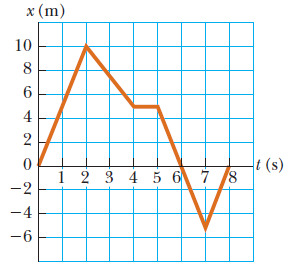
\includegraphics[scale=0.8
    ]{Imagenes/Ejercicio_Cuenta_01.png}
\end{figure}
\end{frame}
\begin{frame}
\frametitle{Enunciado del ejercicio a cuenta}
Encuentra la velocidad en los siguientes intervalos de tiempo:
\setbeamercolor{item projected}{bg=bananayellow,fg=ao}
\setbeamertemplate{enumerate items}{%
\usebeamercolor[bg]{item projected}%
\raisebox{1.5pt}{\colorbox{bg}{\color{fg}\footnotesize\insertenumlabel}}%
}
\begin{enumerate}[<+->]
\item $0$ a \SI{2}{\second}.
\item $0$ a \SI{4}{\second}.
\item $2$ a \SI{4}{\second}.
\item $4$ a \SI{7}{\second}.
\item $0$ a \SI{8}{\second}.
\end{enumerate}
\end{frame}
\begin{frame}
\frametitle{Segundo ejercicio a cuenta}
La posición de un carro de derby se observó en varios momentos; los resultados se resumen en la tabla siguiente.
\pause
\begin{table}
\centering
\begin{tabular}{c | c | c | c | c | c | c}
$t \, (s)$ & $0$ & $1.0$ & $2.0$ & $3.0$ & $4.0$ & $5.0$ \\ \hline
$x \, (m)$ & $0$ & $2.3$ & $9.2$ & $20.7$ & $36.8$ & $57.5$
\end{tabular}
\end{table}
\end{frame}
\begin{frame}
\frametitle{Enunciado del segundo ejercicio}
Encuentra la velocidad del auto para:
\setbeamercolor{item projected}{bg=black,fg=white}
\setbeamertemplate{enumerate items}{%
\usebeamercolor[bg]{item projected}%
\raisebox{1.5pt}{\colorbox{bg}{\color{fg}\footnotesize\insertenumlabel}}%
}
\begin{enumerate}[<+->]
\item El primer intervalo de tiempo de \SI{1}{\second}.
\item Los últimos \SI{3}{\second}
\item Todo el período de observación.
\end{enumerate}
\end{frame}
\begin{frame}
\frametitle{Recomendación}
Es muy recomendable apoyarse con una gráfica de los datos que se presentan en la tabla.
\end{frame}

\section{Movimiento Acelerado}
\frame{\frametitle{Temas a revisar} \tableofcontents[currentsection, hideothersubsections]}
\subsection{Aceleración uniforme}

\begin{frame}
\frametitle{Estudiando la aceleración}
Si la aceleración de un objeto varía con el tiempo, su movimiento es complejo y difícil de analizar.
\\
\bigskip
\pause
Sin embargo, un tipo muy común y simple de movimiento unidimensional, es aquel en el que la \textocolor{firebrick}{aceleración es constante}.
\end{frame}
\begin{frame}
\frametitle{Sobre la velocidad}
En el caso de una aceleración constante, la velocidad cambia con la misma proporción a lo largo del movimiento.
\\
\bigskip
\pause
Esta situación ocurre con suficiente frecuencia como para que se le identifique como un modelo de estudio: un objeto bajo aceleración constante.
\end{frame}
\begin{frame}
\frametitle{Nueva expresión}
De la expresión para la aceleración:
\pause
\begin{align*}
a = \dfrac{v_{f} - v_{i}}{t}
\end{align*}
despejamos la velocidad final $v_{f}$, llegamos a:
\pause
\begin{align*}
\setlength{\fboxsep}{3\fboxsep}\boxed{
v_{f} = v_{i} + a \, t }
\end{align*}
\end{frame}
\begin{frame}
\frametitle{Utilidad de la expresión}
Esta poderosa expresión permite determinar la \textocolor{darkmagenta}{velocidad} de un objeto en cualquier tiempo $t$, si se conoce la velocidad inicial $v_{i}$ del objeto y su aceleración $a$ (constante).
\end{frame}
% \begin{frame}
% \frametitle{Gráfica velocidad contra tiempo}
% A continuación se muestra una gráfica velocidad - tiempo para este movimiento con aceleración
% constante.
% \pause
% \begin{figure}
%     \centering
%     \begin{tikzpicture}
%         \draw (0, 0) -- (6, 0) node [above, pos=1] {$t$};
%         \draw (0, 0) -- (0, 4) node [left, pos=1] {$v$};
%         \draw [line width=0.5mm, color=auburn](0, 1) -- (5, 3);
%         \node at (-0.5, 1) {\small{$v_{i}$}};
%         \draw [dashed] (0, 1) -- (4, 1);
%         \pause
%         \draw [dashed] (4, 0) -- (4, 2.63);
%         \node at (4, -0.3) {\small{$t$}};
%         \pause
%         \draw (4, 2.63) -- (5, 2.63);
%         \draw [<->] (5.2, 0) -- (5.2, 2.63) node [right, midway] {\small{$v_{f}$}};
%         \pause
%         \draw [dashed] (4, 1) -- (5, 1);
%         \draw [<->] (4.2, 0) -- (4.2, 1) node [right, midway] {\small{$v_{f}$}};
%         \pause
%         \draw [<->] (4.2, 1) -- (4.2, 2.63) node [right, midway] {\small{$a \, t$}};
%         \pause
%         \node at (2, 2.3) [rotate=24] {\small{pendiente = $a$}};
%     \end{tikzpicture}
% \end{figure}
% \end{frame}
% \begin{frame}
% \frametitle{Utilidad de la expresión}
% La gráfica es una línea recta, cuya pendiente es la aceleración $a$, \pause recordemos que la pendiente
% es constante.
% \\
% \bigskip
% \pause
% Notemos que la pendiente es positiva, \pause lo que indica una aceleración positiva. \pause Si la aceleración fuese negativa, la pendiente de la recta sería negativa.
% \end{frame}
% \begin{frame}
% \frametitle{Caso de una aceleración constante}
% Cuando la aceleración es constante, la gráfica de aceleración en función del tiempo es una línea recta que tiene una pendiente cero.
% \pause
% \begin{figure}
%     \centering
%     \begin{tikzpicture}
%         \draw (0, 0) -- (6, 0) node [above, pos=1] {$t$};
%         \draw (0, 0) -- (0, 3) node [left, pos=1] {$a$};
%         \draw [line width=0.5mm, color=auburn](0, 1) -- (5, 1);
%         \pause
%         \node at (2, 1.5) {\small{pendiente = $0$}};
%     \end{tikzpicture}
% \end{figure}
% \end{frame}
% \begin{frame}
% \frametitle{Avanzando en el estudio del movimiento}
% Puesto que la velocidad con aceleración constante varía \textocolor{red}{linealmente} en el tiempo, \pause podemos expresar la velocidad promedio en cualquier intervalo de tiempo como la \textocolor{ao}{media aritmética} de la velocidad inicial $v_{i}$ y la velocidad final $v_{f}$:
% \pause
% \begin{align*}
% v = \dfrac{v_{f} - v_{i}}{2}
% \end{align*}
% \end{frame}
% \begin{frame}
% \frametitle{Punto importante}
% Notemos que esta expresión para la velocidad promedio \textocolor{byzantine}{solo} se aplica en situaciones en que la aceleración es constante.
% \end{frame}
% \begin{frame}
% \frametitle{Ocupando una expresión conocida}
% Como ya conocemos la definición de velocidad:
% \pause
% \begin{eqnarray*}
% \begin{aligned}
% v = \dfrac{\Delta x}{t} = \pause \dfrac{x_{f} - x_{i}}{t}
% \end{aligned}
% \end{eqnarray*}
% \pause
% Usamos esta expresión para lo siguiente:
% \end{frame}
% \begin{frame}
% \frametitle{Reescribiendo la expresión}
% Tenemos entonces que:
% \pause
% \begin{eqnarray*}
% \begin{aligned}
% \dfrac{x_{f} - x_{i}}{t} = \pause \dfrac{v_{f} - v_{i}}{2}
% \end{aligned}
% \end{eqnarray*}
% \pause
% Si despejamos $x_{f}$ de la ecuación:
% \end{frame}
% \begin{frame}
% \frametitle{Obteniendo una ecuación nueva}
% Se tiene que:
% \pause
% \begin{eqnarray*}
% \begin{aligned}
% x_{f} - x_{i} &=  \dfrac{1}{2} \, ( v_{f} - v_{i} ) \, t \\[0.5em] \pause
% x_{f} &= x_{i} + \dfrac{1}{2} \, ( v_{f} - v_{i} ) \, t
% \end{aligned}
% \end{eqnarray*}
% Con la aceleración $a$ constante.
% \end{frame}
% \begin{frame}
% \frametitle{Utilidad de la expresión}
% \begin{align*}
% \setlength{\fboxsep}{3\fboxsep}\boxed{
% x_{f} = x_{i} + \dfrac{1}{2} \, ( v_{f} - v_{i} ) \, t }
% \end{align*}
% Esta ecuación nos proporciona la posición final $(x_{f})$ del objeto en el tiempo $t$ en términos de las velocidades inicial $(v_{i})$ y final $(v_{f})$, recordemos que la aceleración es \textbf{constante}.
% \end{frame}
% \begin{frame}
% \frametitle{Ejercicio}
% Un motociclista parte del reposo y experimenta una aceleración de $\SI{2}{\meter\per\square\second}$.
% \\
% \bigskip
% \pause
% ¿Qué distancia habrá recorrido después de $\SI{5}{\second}$?
% \end{frame}
% \begin{frame}
% \frametitle{Expresión a utilizar}
% \begin{align*}
% \setlength{\fboxsep}{3\fboxsep}\boxed{
% x_{f} = x_{i} + \dfrac{1}{2} \, ( v_{f} - v_{i} ) \, t }
% \end{align*}
% Esta ecuación nos proporciona la posición final $(x_{f})$ del objeto en el tiempo $t$ en términos de las velocidades inicial $(v_{i})$ y final $(v_{f})$, recordemos que la aceleración es \textbf{constante}.
% \end{frame}
% \begin{frame}
% \frametitle{Resolviendo el Ejercicio}
% \textbf{Datos:} $v_{i} = 0$, \pause $a = \SI{2}{\meter\per\square\second}$, \pause $t = \SI{4}{\second}$.
% \\
% \bigskip
% \pause
% La expresión a utilizar es:
% \pause
% \begin{align*}
% x_{f} = v_{i} \, t + \dfrac{1}{2} \, a \, t^{2}
% \end{align*}
% \end{frame}
% \begin{frame}
% \frametitle{Resolviendo el Ejercicio}
% Al sustituir los valores que tenemos:
% \begin{eqnarray*}
% \begin{aligned}
% x_{f} &= \dfrac{a \, t^{2}}{2} = \pause \dfrac{\SI{2}{\meter\per\square\second} \, (\SI{4}{\second})^{2}}{2} = \\[0.5em] \pause 
% &= \dfrac{\SI{2}{\meter\per\square\second} \, (\SI{16}{\square\second})}{2} = \\[0.5em] \pause 
% &= \dfrac{\SI{32}{\meter}}{2} = \pause \SI{16}{\meter}
% \end{aligned}
% \end{eqnarray*}
% \end{frame}

\subsection{Ecuaciones de movimiento}

\begin{frame}
\frametitle{Caso con la aceleración constante}
A continuación enlistaremos varias fórmulas que nos permitirán obtener una variable de un objeto que está en movimiento con una \textocolor{carmine}{aceleración constante}.
\end{frame}
\begin{frame}
\frametitle{Ecuaciones de movimiento}
\setbeamercolor{item projected}{bg=firebrick,fg=white}
\setbeamertemplate{enumerate items}{%
\usebeamercolor[bg]{item projected}%
\raisebox{1.5pt}{\colorbox{bg}{\color{fg}\footnotesize\insertenumlabel}}%
}
\begin{enumerate}[<+->]
\item Velocidad como función del tiempo.
\begin{align*}
\setlength{\fboxsep}{3\fboxsep}\boxed{
v_{f} = v_{i} + a \, t
}
\end{align*}
\seti
\end{enumerate}
\end{frame}
\begin{frame}
\frametitle{Ecuaciones de movimiento}
\setbeamercolor{item projected}{bg=firebrick,fg=white}
\setbeamertemplate{enumerate items}{%
\usebeamercolor[bg]{item projected}%
\raisebox{1.5pt}{\colorbox{bg}{\color{fg}\footnotesize\insertenumlabel}}%
}
\begin{enumerate}[<+->]
\conti
\item Posición como función de la velocidad.
\begin{align*}
\setlength{\fboxsep}{3\fboxsep}\boxed{
x_{f} = x_{i} + \dfrac{1}{2} \big( v_{i} + v_{f} \big) \, t
}
\end{align*}
\seti
\end{enumerate}
\end{frame}
\begin{frame}
\frametitle{Ecuaciones de movimiento}
\setbeamercolor{item projected}{bg=firebrick,fg=white}
\setbeamertemplate{enumerate items}{%
\usebeamercolor[bg]{item projected}%
\raisebox{1.5pt}{\colorbox{bg}{\color{fg}\footnotesize\insertenumlabel}}%
}
\begin{enumerate}[<+->]
\conti
\item Posición como función del tiempo.
\begin{align*}
\setlength{\fboxsep}{3\fboxsep}\boxed{
x_{f} = x_{i} + v_{i} \, t + \dfrac{1}{2} a \, t^{2}
}
\end{align*}
\seti
\end{enumerate}
\end{frame}
\begin{frame}
\frametitle{Ecuaciones de movimiento}
\setbeamercolor{item projected}{bg=firebrick,fg=white}
\setbeamertemplate{enumerate items}{%
\usebeamercolor[bg]{item projected}%
\raisebox{1.5pt}{\colorbox{bg}{\color{fg}\footnotesize\insertenumlabel}}%
}
\begin{enumerate}[<+->]
\conti
\item Velocidad como función de la posición
\begin{align*}
\setlength{\fboxsep}{3\fboxsep}\boxed{
v_{f}^{2} = v_{i}^{2} + 2 \, a \big( x_{f} - x_{i}\big)
}
\end{align*}
\end{enumerate}
\end{frame}

\section{Ejercicios de MUA}
\frame{\tableofcontents[currentsection, hideothersubsections]}
\subsection{Ejercicio 1}

\begin{frame}
\frametitle{Ejercicio}
Un jet aterriza en un portaaviones a \SI{63}{\meter\per\second}.
\\
\bigskip
\pause
\textbf{A)} ¿Cuál es su aceleración (constante) si se detiene en \SI{2}{\second} debido a un cable de arresto que traba al jet y lo deja en reposo?
\end{frame}
\begin{frame}
\frametitle{Datos ejercicio}
Leyendo el enunciado de manera cuidadosa, sabemos que la velocidad inicial $v_{i} = \SI{63}{\meter\per\second}$ \pause y que $v_{f} = 0$
\end{frame}
\begin{frame}
\frametitle{Expresión a utilizar}
Con los datos que recuperamos del enunciado, vemos que la siguiente expresión los considera:
\\
\pause
Velocidad como función del tiempo.
\begin{align*}
\setlength{\fboxsep}{3\fboxsep}\boxed{
v_{f} = v_{i} + a \, t
}
\end{align*}
\end{frame}
\begin{frame}
\frametitle{Sutituyendo los datos}
Despejamos la variable $a$ para luego utilizar los datos del enunciado:
\pause
\begin{eqnarray*}
\begin{aligned}
a &= \pause \dfrac{v_{f} - v_{i}}{t} = \\[0.5em] \pause
&= \dfrac{0 - \SI{63}{\meter\per\second}}{\SI{2}{\second}} = \pause - \dfrac{63}{2} = \\[0.5em] \pause
&= \SI{31.5}{\meter\per\second}
\end{aligned}
\end{eqnarray*}
\end{frame}
\begin{frame}
\frametitle{Otro inciso a responder}
\textbf{B)} Si el jet toca al portaaviones en la posición $x_{i} = 0$.
\\
\bigskip
\pause
¿Cuál es su posición final?
\end{frame}
\begin{frame}
\frametitle{Resolviendo el inciso}
Revisamos la lista de expresiones y ocupamos la que considera las variables que ya conocemos:
\\
\pause
Posición como función de la velocidad.
\begin{align*}
\setlength{\fboxsep}{3\fboxsep}\boxed{
x_{f} = x_{i} + \dfrac{1}{2} \big( v_{i} + v_{f} \big) \, t
}
\end{align*}
\end{frame}
\begin{frame}
\frametitle{Sustituimos los valores}
\begin{eqnarray*}
\begin{aligned}
x_{f} &= \pause 0 + \dfrac{1}{2} \big( \SI{63}{\meter\per\second} + 0 \big) \, (\SI{2}{\second}) = \\[0.5em] \pause
&= \SI{63}{\meter\per\second}
\end{aligned}
\end{eqnarray*}
\pause
Si el jet recorre más allá de \SI{63}{\meter}, puede caer al océano.
\end{frame}

\subsection{Ejercicio 2}

\begin{frame}
\frametitle{Enunciado del ejercicio 2}
Un automóvil que viaja con una velocidad constante de \SI{45}{\meter\per\second} pasa por donde un patrullero en motocicleta está oculto
detrás de un anuncio espectacular.
\end{frame}
\begin{frame}
\frametitle{Enunciado del ejercicio 2}
Un segundo después de que el automóvil pasa el anuncio, el patrullero sale de su escondite para detener al automóvil, que acelera con una
relación constante de \SI{33}{\meter\per\square\second}.
\\
\bigskip
\pause
¿Cuánto tiempo tarda en dar alcance al automóvil?
\end{frame}
\begin{frame}
\frametitle{Solución}
Una representación gráfica ayudará a presentar
la secuencia de eventos.
\\
\bigskip
\pause
El automóvil se modela como un objeto bajo \textocolor{ao}{velocidad constante} y el patrullero se modela como un móvil bajo \textocolor{red}{aceleración constante}.
\end{frame}
\begin{frame}
\frametitle{Revisando los eventos}
Primero, escribamos las expresiones para la posición de cada vehículo como función del tiempo.
\\
\bigskip
\pause
Es conveniente elegir la posición del anuncio como el origen y hacer $t_{B} = 0$ como el
tiempo en que el patrullero comienza a moverse. 
\end{frame}
\begin{frame}
\frametitle{Revisando los eventos}
\begin{figure}
    \centering
    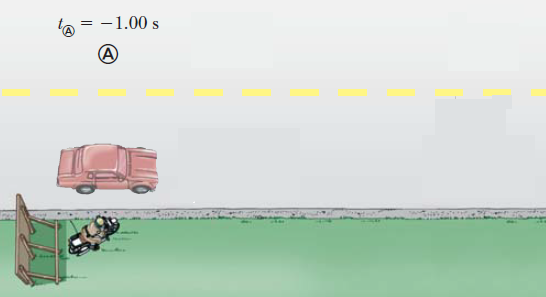
\includegraphics[scale=0.8]{Imagenes/Ejercicio_MUA_02_01.png}
\end{figure}
\end{frame}
\begin{frame}
\frametitle{Revisando los eventos}
En dicho instante, el automóvil ya recorrió una distancia de \SI{45}{\meter} desde el anuncio, \pause porque viajó con una velocidad constante de
$v = \SI{45}{\meter\per\second}$ durante un segundo.
\\
\bigskip
\pause
Por lo tanto, la posición inicial del automóvil es $x_{i} = \SI{45}{\meter}$.
\end{frame}
\begin{frame}
\frametitle{Revisando los eventos}
\begin{figure}
    \centering
    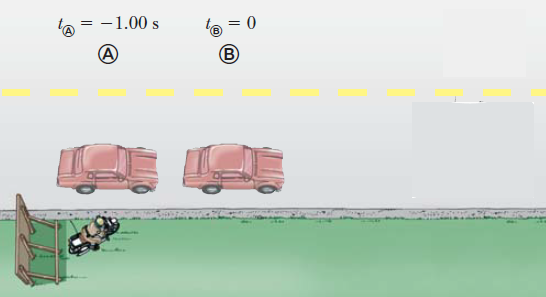
\includegraphics[scale=0.8]{Imagenes/Ejercicio_MUA_02_02.png}
\end{figure}
\end{frame}
\begin{frame}
\frametitle{Posición como función de la velocidad}
Podemos obtener la posición del automóvil en cualquier tiempo $t$:
\pause
\begin{eqnarray*}
\begin{aligned}
x_{\text{auto}} &= x_{B} + v_{\text{auto}} \, t = \\[0.5em] \pause
&= \SI{45}{\meter} + (\SI{45}{\meter\per\second}) \, t
\end{aligned}
\end{eqnarray*}
\end{frame}
\begin{frame}
\frametitle{Estudiando al patrullero}
El patrullero parte del reposo en $t_{B} = 0$ \pause y acelera a $\SI{3}{\meter\per\square\second}$ alejándose del origen.
\\
\bigskip
\pause
Use la siguiente expresión para obtener la posición en cualquier tiempo $t$:
\pause
\begin{align*}
x_{f} = x_{i} + v_{i} \, t + \dfrac{1}{2} a \, t^{2}
\end{align*}
\end{frame}
\begin{frame}
\frametitle{Estudiando al patrullero}
\begin{eqnarray*}
\begin{aligned}
x_{\text{patrulla}} &= 0 + (0) \, t + \dfrac{1}{2} \big( \SI{3}{\meter\per\second} \big) \, t^{2} = \\[0.5em] \pause
&= \dfrac{1}{2} \, \big( \SI{3}{\meter\per\second} \big) \, t^{2}
\end{aligned}
\end{eqnarray*}
\end{frame}
\begin{frame}
\frametitle{Combinando las expresiones}
Iguale las dos posiciones para representar al patrullero dando alcance al automóvil en la posición $C$.
\end{frame}
\begin{frame}
\frametitle{Revisando los eventos}
\begin{figure}
    \centering
    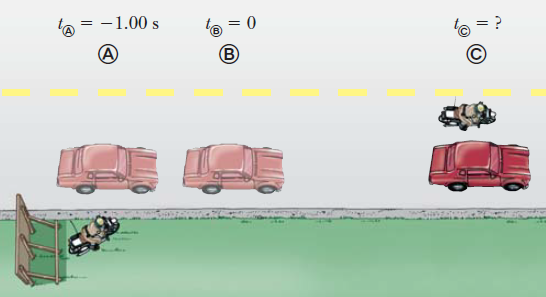
\includegraphics[scale=0.8]{Imagenes/Ejercicio_MUA_02_03.png}
\end{figure}
\end{frame}
\begin{frame}
\frametitle{Igualando las expresiones}
\begin{eqnarray*}
\begin{aligned}
x_{\text{patrulla}} &= x_{\text{auto}} \\[0.5em] \pause
\dfrac{1}{2} \, \big( \SI{3}{\meter\per\second} \big) \, t^{2} &= \SI{45}{\meter} + (\SI{45}{\meter\per\second}) \, t
\end{aligned}
\end{eqnarray*}
\pause
Manejamos el álgebra necesaria para despejar el tiempo $t$.
\end{frame}
\begin{frame}
\frametitle{Simplificando la expresión}
\begin{eqnarray*}
\begin{aligned}
\dfrac{1}{2} \, \big( \SI{3}{\meter\per\second} \big) \, t^{2} &= \SI{45}{\meter} + (\SI{45}{\meter\per\second}) \, t \\[0.5em] \pause
1.5 \, t^{2} - 45 \, t - 45 = 0
\end{aligned}
\end{eqnarray*}
\pause
La última expresión representa una ecuación algebraica de segundo orden, que ya sabemos resolver.
\end{frame}
\begin{frame}
\frametitle{Solución a la ecuación de segundo orden}
\begin{eqnarray*}
\begin{aligned}
1.5 \, &t^{2} - 45 \, t - 45 = 0 \\[0.5em] \pause
t &= \dfrac{- (-45) \pm \sqrt{(-45)^{2} - 4 (1.5)(-45)}}{2 (1.5)} = \\[0.5em] \pause
&= \dfrac{45 \pm \sqrt{2025 - 270}}{3} = \\[0.5em] \pause
&= \dfrac{45 + \sqrt{1755}}{3} = 
\end{aligned}
\end{eqnarray*}
\end{frame}
\begin{frame}
\frametitle{Solución a la ecuación de segundo orden}
\begin{eqnarray*}
\begin{aligned}
t &= \dfrac{45 + 41.89}{3} = \\[0.5em] \pause
&= \dfrac{86.92}{3} = \\[0.5em] \pause 
t &= \SI{28.96}{\second}
\end{aligned}
\end{eqnarray*}
\end{frame}
\end{document}